\documentclass[11pt,a4paper]{article}
\usepackage[a4paper,left=27mm,right=27mm,top=28mm,bottom=30mm,headsep=9mm,footskip=12mm]{geometry}
\usepackage{amsmath}
\usepackage{unicode-math}
\setmainfont{Latin Modern Roman}[Ligatures=TeX]
\setmonofont{Latin Modern Mono}[Scale=0.92]
\setmathfont{Latin Modern Math}
\usepackage{kr}
\usepackage{graphicx,booktabs,tabularx,array,caption,titlesec,fancyhdr,enumitem,xcolor,setspace,ragged2e}
\usepackage[bottom,hang]{footmisc}
\usepackage[hidelinks,unicode]{hyperref}
\usepackage{xurl}

\definecolor{ink}{HTML}{1A1A1A}
\definecolor{note}{HTML}{444444}
\color{ink}
\linespread{1.32}
\setlength{\parindent}{1.2em}
\setlength{\parskip}{0pt}
\setlength{\emergencystretch}{3em}
\setlength{\footnotemargin}{0.9em}
\frenchspacing
\widowpenalty=8000 \clubpenalty=8000

% 제목 체계
\titleformat{\section}{\large\bfseries}{\thesection.}{0.6em}{}
\titleformat{\subsection}{\normalsize\bfseries}{\thesubsection.}{0.6em}{}
\titlespacing*{\section}{0pt}{1.7\baselineskip}{0.6\baselineskip}
\titlespacing*{\subsection}{0pt}{1.2\baselineskip}{0.4\baselineskip}

% 표·그림
\renewcommand{\tablename}{표}
\renewcommand{\figurename}{그림}
\captionsetup{font={small,stretch=1.15},labelfont=bf,labelsep=period,justification=justified,singlelinecheck=false,skip=6pt}
\captionsetup[figure]{position=bottom}
\newcommand{\tnote}[1]{\par\vspace{4pt}{\footnotesize\linespread{1.15}\selectfont\color{note}\justifying\noindent #1\par}}
\newcolumntype{L}[1]{>{\RaggedRight\arraybackslash\hspace{0pt}}p{#1}}
\newcolumntype{Y}{>{\RaggedRight\arraybackslash\hspace{0pt}}X}
\renewcommand{\arraystretch}{1.28}
\setlength{\heavyrulewidth}{0.9pt}\setlength{\lightrulewidth}{0.45pt}
\newcommand{\tablefont}{\small\linespread{1.12}\selectfont}

% 머리말
\pagestyle{fancy}\fancyhf{}
\renewcommand{\headrulewidth}{0.3pt}
\fancyhead[L]{\footnotesize\color{note} 박찬진}
\fancyhead[R]{\footnotesize\color{note} 실행되지 않는 위협의 발표효과}
\fancyfoot[C]{\small\thepage}
\fancypagestyle{first}{\fancyhf{}\renewcommand{\headrulewidth}{0pt}\fancyfoot[C]{\small\thepage}}

\newcommand{\Bcit}{B^{\mathrm{cit}}}
\newcommand{\Bfam}{B^{\mathrm{fam}}}
\newcommand{\pp}{\%p}
\newcommand{\hyp}[1]{\textbf{H#1}}


\usepackage{float}
\begin{document}
\thispagestyle{first}
\begin{center}
{\LARGE\bfseries 실행되지 않는 위협의 발표효과\par}
\vspace{9pt}
{\large 관세 위협과 수출통제 예고에 대한 고빈도 사건연구, 2025--2026\par}
\vspace{20pt}
{\large 박찬진\footnote{KAIST. 사건 목록과 분석계획(v1.1)은 가격 자료를 열람하기 전에 고정했고, 그 해시와 이후의 변경 이력을 재현자료에 보존했다. 5절의 검정은 사전에 정한 것이고 6--7절의 분석은 결과를 본 뒤에 추가한 탐색적 분석이다. 본문에서 두 종류를 구분해 표시한다.}\par}
\vspace{6pt}
{\normalsize 2026년 11월 15일\par}
\end{center}

\vspace{12pt}
\begin{center}
\begin{minipage}{0.9\textwidth}
\small\linespread{1.25}\selectfont
\begin{center}\textbf{초록}\end{center}
\noindent 발표효과 연구는 약속을 지킨다고 여겨지는 발표자를 다뤄 왔다. 본 연구는 반대의 경우, 곧 위협의 대부분을 실행하지 않는 발표자를 다룬다. 2025년 1월부터 2026년 7월까지 미국 대통령의 관세 강화 위협 33건, 완화·철회 13건, 예정 발효 11건을 가격 자료를 보기 전에 목록으로 고정하고, 게시 시각을 원문으로 확인한 40건에 대해 분 단위 주가지수와 대상국 통화의 반응을 같은 시각 비사건 창으로 표준화했다. 결과가 확정된 위협 32건 중 예고대로 실행된 것은 7건(22\%)이다. 그럼에도 (1) 위협 20건 중 16건에서 가격은 위험회피 방향으로 움직였고 평균 반응은 표준편차의 0.59배였으며, 이 크기는 표본 전반과 후반 사이에 줄지 않았다. (2) 발표 시점의 반응은 나중에 실행된 위협과 실행되지 않은 위협 사이에 차이가 없었다. (3) 철회에는 반대 방향으로 반응했고($-0.91$), 예정된 발효일에는 반응하지 않았다($0.17$). 탐색적 분석은 이 결과를 세 층으로 설명한다. 첫째, 미실행은 한 종류가 아니다. 협상이나 상대의 양보로 끝난 위협은 발표 때 크게 반응했고(평균 1.52), 번복 발표 없이 사라진 위협은 처음부터 거의 반응이 없었다(0.26). 둘째, 예측시장은 특정 위협의 실행 확률을 평균 0.44로 매겼고 실제 실행 비율은 0.38이었다. 시장은 위협을 믿지 않은 것이 아니라 낮은 실행 확률만큼만 반영했다. 셋째, 2025년 이후 수출통제 예고 때 중국 국산 대체 기업의 주가는 미국 공급사 대비 평균 2.7\pp 올랐고 번복 때 2.3\pp 내렸다. 표본이 작아 집단 간 비교의 검정력은 낮으며, 본 연구는 그 한계 안에서 실행률이 신뢰도의 척도가 아니라는 점과, 발표효과가 실행 실적이 아니라 실행 능력과 판의 크기에 달려 있다는 해석을 제시한다.

\vspace{6pt}
\noindent\textbf{주제어}: 발표효과, 관세 위협, 신뢰도, 사건연구, 예측시장, 수출통제\\
\textbf{JEL}: F13, G14, G12, D83, F51
\end{minipage}
\end{center}
\vspace{6pt}

\section{서론}

2020년 3월 23일 연방준비제도는 회사채 매입기구 두 개를 발표했다. 투자등급 회사채 가격은 발표 시점에 약 7\% 올랐다\,(Haddad, Moreira and Muir, 2021). 그런데 발행시장 매입기구(PMCCF)는 한 건도 매입하지 않고 종료됐다. 시장을 되돌린 것은 매입이 아니라 매입하겠다는 말이었다. 양적완화, 포워드 가이던스, 유럽중앙은행의 OMT까지, 발표효과 연구의 대표 사례는 모두 같은 조건 위에 서 있다. 발표자가 약속을 지킬 것이라고 시장이 믿었다는 조건이다.

본 연구는 이 조건이 성립하지 않는 경우를 다룬다. 2025년 1월 이후 미국 대통령은 수십 차례 관세를 올리겠다고 위협했고, 그중 다수를 실행하지 않았다. 본 연구가 고정한 목록에서 결과가 확정된 강화 위협 32건 중 예고대로 실행된 것은 7건이고, 부분 실행 4건을 더해도 11건(34\%)이다. 발표자가 반복해서 말을 거두는 환경에서 말은 여전히 가격을 움직이는가. 움직인다면 시장은 어떤 위협을 얼마나 믿는가. 이것이 본 연구의 질문이다.

이 질문은 세 가지 이유로 중요하다. 첫째, 위협은 실행 비용 없이 협상력을 얻는 수단이므로 시장이 반응하지 않게 되면 수단 자체가 사라진다. 둘째, 관세 발표에 대한 기존 사건연구는 위협과 시행을 구분하지 않거나 시행된 조치만 다룬다. 실행되지 않은 위협은 사후에 ``아무 일도 없었던 날''로 남아 표본에서 빠지기 쉽다. 셋째, 같은 발표자가 짧은 기간에 수십 번 위협했고 각 위협의 결말이 관측되므로, 발표효과가 발표자의 실행 실적에 따라 어떻게 달라지는지를 처음으로 사건 단위에서 볼 수 있다.

본 연구의 접근은 세 가지다. 먼저 사건 57건과 각 위협의 실행 여부를 가격과 무관한 규칙으로 코딩해 가격을 보기 전에 고정했다. 다음으로 게시 시각을 원문 기록으로 확인하고, 분 단위 S\&P 500과 대상국 통화의 반응을 같은 요일·같은 시각의 비사건 창으로 표준화했다. 마지막으로 사건 수에 맞는 질문만 던졌다. 실행률에 대한 기울기 회귀는 검정력이 없다는 것을 모의자료로 먼저 확인했고, 주 검정을 평균과 집단 대비로 바꿨다.

사전에 정한 검정의 결과는 네 가지다. 위협은 여전히 시장을 움직이지만 크기는 작다. 그 크기는 표본 기간인 약 1년 동안 줄지 않았다. 발표 시점의 반응은 실행될 위협과 아닌 위협을 가르지 못했다. 철회에는 반응하고 발효일에는 반응하지 않았다.

이 결과만으로는 ``시장이 모든 위협을 비슷하게 의심했다''고 읽기 쉽다. 결과를 본 뒤 추가한 분석은 그 읽기가 틀렸음을 시사한다. 미실행 21건을 사유별로 나누면, 협상 타결이나 상대의 양보로 끝난 위협은 발표 때 가장 크게 반응했고, 번복 발표도 없이 시한만 지나 사라진 위협은 처음부터 반응이 없었다. 예측시장 계약 32건은 특정 위협의 실행 확률을 평균 0.44로 매겼고 실제 실행 비율은 0.38이었다. 시장은 위협을 종류별로 가려 들었고, 낮은 실행 확률을 대체로 맞게 가격에 반영했다. 전체 실행률이 낮다는 사실과 발표효과가 유지된다는 사실은 그래서 모순이 아니다.

본 연구는 원래 다른 질문에서 출발했다. 2018년 미국의 신흥기술 수출통제 예고가 중국의 연구배분을 바꿨는지를 특허 자료로 식별하려 했고, 그 시도는 실패했다. 3절은 실패의 이유를 기록한다. 그 실패가 지금의 설계를 정했기 때문이다. 7절은 처음의 질문으로 돌아가, 수출통제 예고와 번복이 자본의 방향에 대한 시장의 기대를 움직였는지를 주가로 본다.

\section{관련 연구와 본 연구의 위치}

\textbf{발표효과.} 자산매입 발표일의 장기금리 하락\,(Krishnamurthy and Vissing-Jorgensen, 2011), 정책금리 결정과 구분되는 성명 문구의 효과\,(Gürkaynak, Sack and Swanson, 2005), 발동된 적 없는 OMT의 국채금리 효과\,(Altavilla, Giannone and Lenza, 2016), 회사채 매입기구 발표의 효과\,(Haddad, Moreira and Muir, 2021)는 실행 이전의 말이 가격을 움직인다는 것을 보였다. 이 연구들에서 발표자의 신뢰도는 높고 대체로 일정하다. 본 연구는 신뢰도가 낮고 사건마다 다른 발표자를 다룬다.

\textbf{관세 발표의 사건연구.} 2018--2019년 관세 발표일의 주가 반응은 Amiti, Gomez, Kong and Weinstein\,(2021) 등이 다뤘다. 2025년 이후에 대해서는 Kalemli-Özcan, Soylu and Yildirim\,(2026)이 시각이 찍힌 사건 319건을 177개 묶음으로 정리하고 분 단위 반응을 추정했다. 이 연구는 위협과 시행을 나누지 않고, 반응이 시간에 따라 또는 실행 실적에 따라 달라지는지를 검정하지 않으며, 예측시장을 쓰지 않는다. Merendino and Monacelli\,(2026)는 관세의 지속성에 대한 학습을 분기 단위 모형으로 다룬다. 본 연구는 사건 단위에서 위협, 철회, 발효를 구분하고 각 위협의 결말을 붙였다.

\textbf{위협의 실행률.} 경제제재 문헌은 위협과 부과를 따로 기록한다. TIES 자료의 1,412건 중 제재가 실제로 부과된 것은 845건(60\%)이고, 위협 단계에서 끝난 사례의 절반가량은 상대의 양보로 끝났다\,(Morgan, Bapat and Kobayashi, 2014). 미국 통상법 301조 사건 91건(1975--1994) 중 일방적 보복이 단행된 것은 12건이다\,(Bayard and Elliott, 1994). 실행되지 않은 위협이 곧 실패한 위협은 아니라는 이 문헌의 구분을 본 연구는 6절에서 사건별 시장 반응에 적용한다.

\textbf{수출통제와 혁신.} 통제 대상국의 연구개발 반응에 대한 추정은 엇갈린다. Liu, Liu, Makarin and Wen\,(2025)은 2007년 대중 통제 이후 대상 품목 수입 기업의 연구개발비가 49\% 늘었다고 추정하고, Hu, Yang, Zeng and Zhang\,(2024)은 Entity List 등재 기업의 연구개발 집약도 증가와 산출의 정체를 보고하며, Hayakawa and Yang\,(2026)은 증가가 없다고 보고한다. Ma, Ma, Tao and Zhang\,(2025)은 관세가 특허와 연구개발비를 줄였다고 추정한다. 이 연구들은 시행된 조치와 연간 연구개발 수준을 본다. 예고만 있고 번복된 통제에 대한 반응은 다뤄지지 않았다.

\section{첫 시도와 실패: 2018년 수출통제 예고와 특허}

처음의 질문은 2018년 11월 미국 상무부의 신흥기술 수출통제 사전예고(ANPRM)가 실제 통제 이전에 중국의 자체 연구를 늘렸는가였다. 단순한 모형에서 규제 확률 $p$가 오르면 기업가치는 항상 떨어지지만, 자체 연구투자 $I^{*}$의 방향은 미국 기술과 자체 연구가 대체재인지 보완재인지에 달려 정해지지 않는다. 주가만으로는 연구의 방향을 알 수 없으므로 특허로 직접 보려 했다. 18개 기술, 5개국, 120개월의 특허 패널에서 예고가 지목한 기술과 지목하지 않은 기술을, 사전 미국 의존도에 따라 비교하는 설계였다.

이 설계는 세 가지 이유로 성립하지 않았다.

\textbf{비교 대상의 부재.} 지목 기술(인공지능, 음성인식, 적층제조 등)과 비지목 기술(성형, 절삭, 연삭)의 미국 의존도 범위는 한 곳도 겹치지 않았다. 대체 지표로 겹치는 구간을 만들면 지목 2개, 비지목 3개 기술만 남았다. 지목된 기술은 처음부터 다른 종류의 기술이었다.

\textbf{가짜 시점.} 실제 창(2018년 12월--2019년 4월)의 추정치는 $-0.359$였는데, 아무 신호가 없던 2013--2015년의 같은 달 창에서는 $-1.1$에서 $-1.3$이 나왔다. 의존도를 4,999번 재배정한 분포에서도 실제 추정치는 이례적이지 않았다. 추정치가 잡은 것은 정책이 아니라 의존도가 높은 기술일수록 빨랐던 추격 추세였다.

\textbf{사전 추세.} 지목과 비지목의 차등 기울기는 2010--2017년 사이에 $+3$에서 $-2$까지 움직였고, 2018년 전후로 달라진 패턴이 없었다. 연구에서 출원까지의 시차를 생각하면 5개월 창으로 반응을 잡는 것도 무리였다.

판정은 이 설계로 연구배분의 인과효과를 말할 수 없다는 것이다. 효과가 없다는 증거도 아니다. 이 실패에서 세 가지를 가져왔다. 신호는 한 번에 오지 않고 보고서, 입법, 예고, 시행이 따로 도착하므로 예고와 시행을 구분해야 한다. 설계는 가짜 시점과 재배정으로 먼저 깨 봐야 한다. 그리고 질문을 한 단계 앞으로 줄여야 한다. 예고가 연구를 바꿨는지를 묻기 전에, 예고가 정보로서 시장에 도착했는지부터 확인해야 한다.

두 번째 시도는 사건 하나였다. 2025년 10월 10일 10시 57분(미 동부시각) 대통령이 대중 관세 인상을 위협했고, 그 시각을 포함한 한 시간 동안 중국 ADR 4개사는 시장조정 후 4.03\% 하락했다. 과거 59거래일의 같은 시각 중 가장 큰 하락이었다. 여기서 두 가지를 더 배웠다. 그날 보도의 제목이 된 ``100\% 관세와 소프트웨어 수출통제''는 16시 50분, 장 마감 후에 게시됐다. 정규장의 하락은 그보다 앞선 위협에 대한 반응이었고, 일별 자료로는 둘을 구분할 수 없다. 게시 시각을 원문으로 확인하고 분 단위로 맞추는 것이 설계의 첫 규칙이 됐다. 그리고 사건 하나로는 아무것도 일반화할 수 없다. 이것이 사건 패널로 넘어간 이유다.

\section{자료와 설계}

\subsection{사건 패널}

사건은 세 종류다. 강화 위협은 대통령이 아직 시행되지 않은 관세 인상을 공개적으로 예고한 것, 완화·철회는 예고했거나 시행 중인 관세의 유예·인하·철회를 알린 것, 예정 발효는 미리 공표된 일정대로 관세가 발효된 시점이다. 2025년 1월부터 2026년 7월까지 강화 위협 33건, 완화·철회 13건, 예정 발효 11건을 수집했다. 목록은 전수가 아니며, 서한이나 기자회견 발언으로만 나온 위협은 시각을 특정할 수 없어 대부분 빠져 있다.

게시 시각은 American Presidency Project가 보존한 Truth Social 일별 기록에서 확인했다. 기록의 태평양시각 표기를 동부시각으로 변환했다. 시각이 확인된 사건은 강화 위협 21건, 완화·철회 9건, 예정 발효 11건이고, 가격 자료가 닿는 범위에서 분석에 쓴 것은 각각 20건, 9건, 11건이다. 시각을 확인하지 못한 강화 위협 12건은 실행률 계산에만 쓴다.

각 위협의 결말은 가격과 무관한 규칙으로 코딩했다. 예고한 시한이 있으면 그 시한에 예고한 내용이 발효됐는지를 본다. 시한이 없으면 90일 안에 발효됐는지를 본다. 나중에 다른 법적 근거로 비슷한 조치가 나와도 원래 위협의 결말은 바꾸지 않는다. 세율이나 범위가 줄어든 채 발효되면 부분 실행이다. 그 결과 강화 위협 33건은 실행 7건, 부분 실행 4건, 미실행 21건, 미확정 1건으로 나뉜다(표~\ref{t:panel}). 결말의 근거는 관세 추적 자료와 통신사 연표이며 사건별로 기록했다.

\begin{table}[H]
\caption{사건 패널}\label{t:panel}
\tablefont
\begin{tabularx}{\textwidth}{@{}Yrrr@{}}
\toprule
 & 강화 위협 & 완화·철회 & 예정 발효\\
\midrule
수집한 사건 & 33 & 13 & 11\\
게시 시각 확인 & 21 & 9 & 11\\
분 단위 분석에 사용 & 20 & 9 & 11\\
\midrule
\multicolumn{4}{@{}l}{강화 위협의 결말 (33건)}\\
\quad 실행 & 7 & & \\
\quad 부분 실행 & 4 & & \\
\quad 미실행 & 21 & & \\
\quad 미확정 & 1 & & \\
\bottomrule
\end{tabularx}
\tnote{주: 사건 목록(v1)은 가격 자료 열람 전에 고정했다. 결말이 확정된 32건 기준 실행 비율은 22\%, 부분 실행을 포함하면 34\%다.}
\end{table}

실행 실적의 지표로는 각 사건 시점까지 결말이 확정된 과거 위협만으로 계산한 실행 비율의 Beta(1,1) 사후평균을 썼다(그림~\ref{f:cred}). 이 값은 2025년 내내 0.40--0.46에 머물렀고 2026년에 0.31로 내려갔다. 실행률은 처음부터 낮았고 표본 기간 안에서 크게 변하지 않았다. 이 점이 뒤에서 기울기 회귀를 주 검정에서 뺀 이유다.

\begin{figure}[H]
\centering
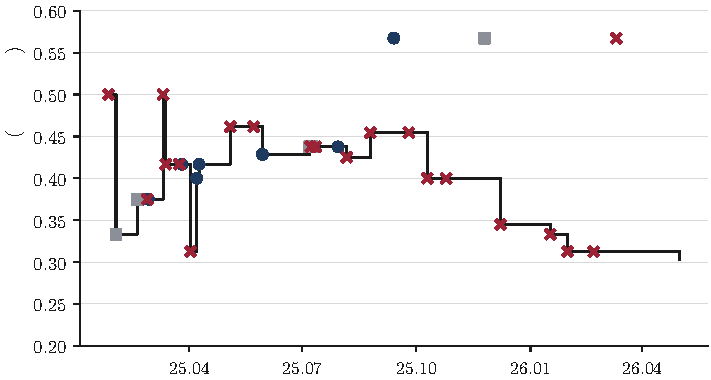
\includegraphics[width=0.72\textwidth]{fig/cred_path.pdf}
\caption{강화 위협의 누적 실행 비율. 각 시점까지 결말이 확정된 과거 위협으로 계산한 Beta(1,1) 사후평균이다.}\label{f:cred}
\end{figure}

\subsection{반응의 측정}

가격은 Dukascopy의 1분봉이다. 시장 전체의 반응은 S\&P 500 지수 CFD로, 대상국 고유의 반응은 대상국 통화의 달러 환율로 잰다. 사건 $i$의 반응은 게시 5분 전부터 30분 후까지의 로그수익률이며, 부호는 위험회피 방향이 양(+)이 되도록 맞췄다. S\&P 500은 하락이, 대상국 통화는 약세가 양이다.

수익률은 같은 요일, 같은 시각의 비사건 창 20--60개에서 구한 표준편차로 나눠 표준화한다. 시각대에 따라 변동성이 크게 다르기 때문이다. 대상국 통화가 있는 사건은 두 표준화 반응의 평균을, 없는 사건은 S\&P 500의 표준화 반응을 종합 반응 $z_i$로 쓴다. 시장이 닫혀 있을 때 게시된 사건은 휴장 직전 가격에서 재개장 30분 후 가격까지를 재고, 비사건 창도 같은 방식으로 구성한다. 창의 길이를 15, 60, 120분으로 바꾼 결과와 휴장 사건을 뺀 결과는 5.5절에 보고한다.

\subsection{검정}

단순한 학습 모형에서 위협에 대한 가격 반응은 대략 $\Delta p \times L$이다. $\Delta p$는 발표가 실행 확률을 얼마나 올렸는가이고 $L$은 실행됐을 때의 손실이다. 이 틀에서 세 가지를 예측할 수 있다. 시장이 위협을 덜 믿으면 발표 시점의 반응이 작다(P1). 이 경우 발효가 새 정보이므로 발효 시점의 반응은 커야 한다(P2). 그리고 처음에 덜 반영됐으므로 철회 시점에 되돌릴 것도 적다(P3). P2가 중요한 것은 ``시장이 관세 뉴스에 무뎌졌다''는 대안 설명과 갈리는 지점이기 때문이다. 무뎌진 것이라면 발효일의 반응도 작아야 한다.

분석계획(v1)은 실행 비율에 대한 반응의 기울기를 주 검정으로 뒀다. 실제 가격을 보기 전에 모의자료로 점검한 결과, 통화 반응만 쓰는 설계에서는 쓸 수 있는 위협이 9건뿐이고 실행 비율의 범위가 0.29--0.50으로 좁아 기울기 회귀의 검정력이 없었다. 그래서 가격을 보기 전에 계획을 고쳤다(v1.1). 시장 전체의 반응을 결과 변수에 추가하고, 주 검정을 다음 네 가지 평균·대비 검정으로 바꿨다.

\begin{itemize}[leftmargin=2.2em,itemsep=1pt,topsep=3pt]
\item[T1] 강화 위협의 평균 반응이 0인가, 표본 전반과 후반의 평균이 같은가
\item[T2] 나중에 실행된 위협과 실행되지 않은 위협의 발표 시점 반응이 같은가
\item[T3] 예정 발효의 평균 반응이 0인가, 그 절대 크기가 위협보다 큰가
\item[T4] 완화·철회의 평균 반응이 0인가
\end{itemize}

집단 간 차이는 순열 검정과 순위합 검정으로, 평균은 표본 $t$ 통계량과 부호 검정으로 판단한다. 기울기 회귀는 보조 분석으로 남기고 최소검출효과와 함께 보고한다.

\section{결과}

\subsection{위협은 여전히 시장을 움직인다}

강화 위협 20건의 평균 표준화 반응은 0.59, 중앙값은 0.36이다(표~\ref{t:main}, 그림~\ref{f:esc}). 20건 중 16건이 위험회피 방향이다(부호 검정 $p=0.012$). 표본 $t$ 통계량은 1.40으로 통상의 유의수준에 못 미치는데, 한 사건이 평균을 크게 끌어내리기 때문이다. 2025년 4월 9일의 대중 125\% 위협은 상호관세 90일 유예와 같은 게시물에 들어 있었고 시장은 유예에 반응했다($z=-4.74$). 이 혼합 사건을 빼면 평균은 0.87, $t=2.64$다.

크기는 작다. 위협 직후 30분 동안 S\&P 500의 중앙값 변화는 $-0.09$\%다. 전형적인 위협은 그 시각대 평소 변동의 절반 남짓만큼 가격을 움직였다.

\begin{table}[H]
\caption{주 결과: 사건 유형별 표준화 반응}\label{t:main}
\tablefont
\begin{tabularx}{\textwidth}{@{}Yrrrrr@{}}
\toprule
 & 건수 & 평균 $z$ & 중앙값 & 표본 $t$ & 예상 부호 건수\\
\midrule
강화 위협 & 20 & $0.59$ & $0.36$ & $1.40$ & 16\\
\quad 4/9 혼합 사건 제외 & 19 & $0.87$ & & $2.64$ & 16\\
\quad 표본 전반 10건 & 10 & $0.45$ & & & \\
\quad 표본 후반 10건 & 10 & $0.73$ & & & \\
완화·철회 & 9 & $-0.91$ & & $-2.15$ & 7\\
\quad 4/9 유예 제외 & 8 & $-0.59$ & & $-1.87$ & 6\\
예정 발효 & 11 & $0.17$ & & $0.74$ & \\
\midrule
\multicolumn{6}{@{}l}{위협의 결말별 (발표 시점 반응)}\\
\quad 실행·부분 실행 & 6 & $-0.32$ & & & \\
\quad\quad 4/9 혼합 사건 제외 & 5 & $0.56$ & & & \\
\quad 미실행 & 14 & $0.98$ & & & \\
\bottomrule
\end{tabularx}
\tnote{주: 반응은 게시 5분 전부터 30분 후까지의 로그수익률을 같은 요일·시각 비사건 창의 표준편차로 나눈 값이며 위험회피 방향이 양이다. 전반·후반 차이의 순열 검정 $p=0.74$. 실행 대 미실행 차이의 순열 검정 $p=0.19$, 혼합 사건 제외 시 순위합 검정 $p=0.82$.}
\end{table}

\begin{figure}[H]
\centering
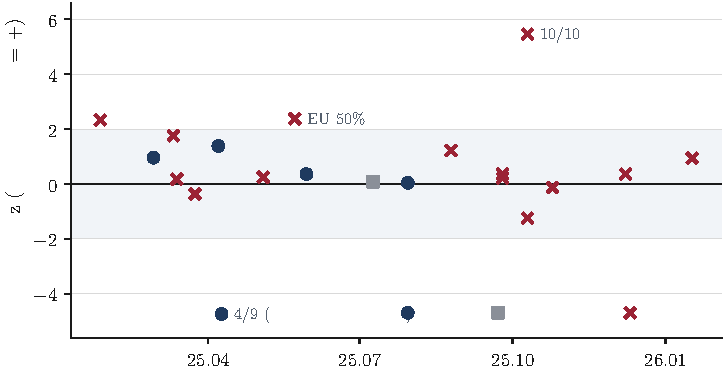
\includegraphics[width=0.78\textwidth]{fig/res_esc_scatter.pdf}
\caption{강화 위협 20건의 표준화 반응. 음영은 $\pm1.96$ 구간이다.}\label{f:esc}
\end{figure}

\subsection{시간이 지나도 줄지 않았다}

표본을 시간순으로 반으로 나누면 전반 10건(2025년 1--5월)의 평균은 0.45, 후반 10건(2025년 7월--2026년 1월)의 평균은 0.73이다. 차이의 순열 검정 $p$값은 0.74다. 실행되지 않은 위협이 쌓이는 동안 반응이 약해졌다는 증거는 없다. 보조 분석인 기울기 회귀에서 누적 실행 비율의 계수는 5.5(표준오차 6.8)이고, 이 표본에서 80\% 검정력으로 잡을 수 있는 최소 기울기는 약 28이다. 실행 비율의 범위가 좁아 이 회귀는 어느 쪽으로도 말해 주는 것이 없다.

\subsection{실행될 위협을 가려내지 못했다}

나중에 실행되거나 부분 실행된 위협 6건의 발표 시점 평균 반응은 $-0.32$, 실행되지 않은 14건의 평균은 0.98이다. 혼합 사건을 빼면 실행 집단의 평균은 0.56이고 차이는 유의하지 않다(순위합 $p=0.82$). 가장 큰 반응 두 건, 곧 2025년 10월 10일의 대중 위협과 5월 23일의 EU 50\% 위협은 모두 실행되지 않았다. 반대로 실행된 인도 25\%와 구리 50\%는 발표 때 지수와 환율이 거의 움직이지 않았다. 실행 집단이 5--6건이라 이 비교의 검정력은 낮다.

\subsection{철회에는 반응하고 발효일에는 반응하지 않는다}

완화·철회 9건의 평균 반응은 $-0.91$($t=-2.15$)이고 7건이 위험선호 방향이다. 4월 9일 유예를 빼도 $-0.59$($t=-1.87$)다. 철회 직후 30분 S\&P 500의 중앙값 변화는 $+0.44$\%로, 위협 때의 $-0.09$\%보다 크다. 예정 발효 11건의 평균은 0.17($t=0.74$), S\&P 500 중앙값 변화는 0.00\%다. 발효의 절대 반응이 위협보다 크다는 증거는 없고(순열 $p=0.12$), 통화 반응만 보면 발효 쪽이 오히려 작다($p=0.028$).

세 예측에 비춰 보면 P1은 맞고(반응이 작다) P2와 P3는 틀렸다. 발효일에 새 정보가 도착하지 않았고, 철회에는 분명한 반응이 있었다. 위협이 발표 때 조금만 반영되고 나머지는 발효 때 반영된다는 단순한 그림은 자료와 맞지 않는다. 발효 여부는 발효일 이전에, 발표와 철회 사이의 어느 시점에 이미 해소돼 있었다.

\subsection{강건성}

표~\ref{t:rob}은 정의를 바꾼 결과다. 창을 15분으로 줄이면 위협의 평균 반응은 0.83으로 커지고 120분으로 늘리면 0.37로 줄어든다. 반응이 게시 직후에 집중돼 있다는 뜻이며, 분 단위 자료가 아니면 보이지 않는 크기다. 게시 전에 내용이 일부 알려졌던 사건, 휴장 중 게시된 사건, 2025년 4월 2--9일의 사건을 각각 빼도 세 유형의 부호는 같다. 실행 비율의 정의 4종, 부분 실행의 가중치(0, 0.5, 1), 시한 규칙(60, 90, 120일)을 바꿔도 기울기는 어느 명세에서도 유의하지 않다.

\begin{table}[H]
\caption{강건성: 유형별 평균 표준화 반응}\label{t:rob}
\tablefont
\begin{tabularx}{\textwidth}{@{}Yrrr@{}}
\toprule
명세 & 강화 위협 (건수) & 완화·철회 & 예정 발효\\
\midrule
주 명세 [$-5$, $+30$]분 & $0.59$ (20) & $-0.91$ & $0.17$\\
창 [$-5$, $+15$]분 & $0.83$ (20) & $-0.76$ & $0.11$\\
창 [$-5$, $+60$]분 & $0.47$ (20) & $-0.80$ & $0.18$\\
창 [$-5$, $+120$]분 & $0.37$ (20) & $-0.43$ & $0.12$\\
사전에 알려진 사건 제외 & $0.42$ (18) & $-0.90$ & $0.17$\\
휴장 중 게시 제외 & $0.63$ (15) & $-1.07$ & $0.17$\\
2025.4.2--4.9 제외 & $0.84$ (18) & $-0.59$ & $0.28$\\
\bottomrule
\end{tabularx}
\end{table}

\section{해석: 낮은 실행률과 유지되는 발표효과는 어떻게 공존하는가}

이 절의 분석은 5절의 결과를 본 뒤에 추가했다. 분류는 가격과 무관한 공개 기록에 근거했지만 분류 기준 자체를 사후에 정했으므로, 아래의 수치는 가설을 세우는 근거로 읽어야 한다.

\subsection{미실행은 한 종류가 아니다}

실행되지 않은 위협 21건을 결말에 이른 경로로 나눴다. 상대국이 요구를 받아들여 위협을 실행할 필요가 없어진 경우(상대 양보, 4건), 협상으로 더 낮은 세율이나 휴전에 합의한 경우(협상 타결, 5건), 상대의 양보가 확인되지 않은 채 보류되거나 사라진 경우(일방 보류·소멸, 12건)다. 법원의 판결로 막힌 위협은 이 목록에 없다. 드러난 방식으로 보면 11건은 번복이나 합의가 명시적으로 발표됐고, 10건은 아무 발표 없이 시한만 지났다.

\begin{table}[H]
\caption{위협의 결말별 발표 시점 반응 (사후 분류)}\label{t:reason}
\tablefont
\begin{tabularx}{\textwidth}{@{}Yrrrr@{}}
\toprule
 & 건수 & 평균 $z$ & 중앙값 & S\&P 500 중앙값 (\%)\\
\midrule
협상으로 낮춰 타결 & 4 & $1.88$ & $1.66$ & $-0.95$\\
상대의 양보 & 4 & $1.15$ & $1.06$ & $-0.42$\\
실제 실행 (4/9 제외) & 5 & $0.56$ & $0.36$ & $-0.08$\\
일방적 보류·소멸 & 6 & $0.26$ & $0.23$ & $-0.05$\\
\midrule
미실행 중 명시적 번복·합의 & 9 & $1.39$ & $0.94$ & \\
미실행 중 발표 없이 소멸 & 5 & $0.23$ & $0.17$ & \\
\bottomrule
\end{tabularx}
\tnote{주: 시각이 확인된 강화 위협 가운데 반응을 잰 사건이다. 협상·양보 8건 대 일방 소멸 6건의 순열 검정 $p=0.16$, 순위합 $p=0.18$. 명시 대 소멸의 순위합 $p=0.11$. S\&P 500 열은 30분 수익률이다.}
\end{table}

표~\ref{t:reason}과 그림~\ref{f:reason}이 결과다. 협상이나 양보로 끝난 위협 8건의 발표 시점 평균 반응은 1.52이고, 일방적으로 보류되거나 사라진 6건은 0.26이다. 실제로 실행된 위협은 그 사이에 있다. 차이는 통계적으로 유의하지 않지만 순서는 분명하다. 시장이 가장 크게 반응한 위협은 실행되지 않았고, 그 이유는 위협이 약해서가 아니라 협상의 대상이 될 만큼 컸기 때문으로 보인다. 반대로 조용히 사라질 위협은 발표 때부터 거의 무시됐다.

\begin{figure}[H]
\centering
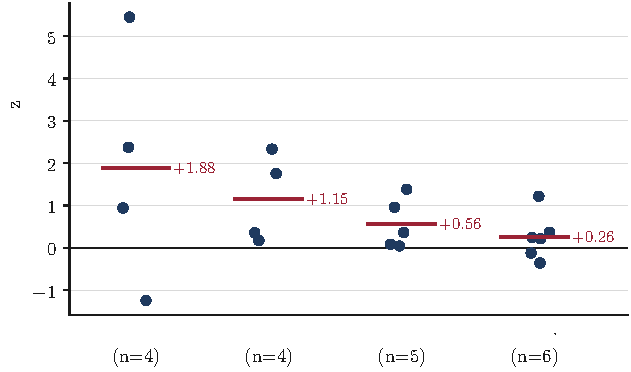
\includegraphics[width=0.66\textwidth]{fig/int_reason.pdf}
\caption{위협의 결말별 표준화 반응. 가로선은 집단 평균이다. 4월 9일 혼합 사건은 제외했다.}\label{f:reason}
\end{figure}

이 결과에는 측정의 한계가 있다. 일방 소멸 집단에는 영화, 의약품, 트럭 같은 품목 관세가 많고, 품목 관세는 지수나 환율이 아니라 해당 품목의 가격에 반영된다. 구리 50\% 관세가 예고된 2025년 7월 8일 미국 구리 선물은 12.4\% 올랐지만 S\&P 500의 표준화 반응은 0.08이었다. 의약품 100\% 관세가 예고된 다음 날 제약 ETF는 시장보다 2.0\pp 더 올랐는데, 미국 내 생산 기업을 면제하는 조건이 붙어 있었기 때문이다. 그러므로 ``시장이 이 위협들을 무시했다''는 표현은 시장 전체 지표에 한해서만 성립한다.

두 가지 함의가 있다. 하나는 실행률이 신뢰도의 척도가 아니라는 것이다. 미실행 21건 중 9건은 위협이 통해서 실행할 필요가 없어진 경우이고, 나머지 상당수는 시장이 처음부터 크게 반영하지 않은 위협이다. 전체 실행 비율로 만든 신뢰도 지표가 반응을 설명하지 못한 것(5.2절)은 이 지표가 서로 다른 것을 한데 섞었기 때문일 수 있다. 다른 하나는 5.3절의 ``가려내지 못했다''를 고쳐 읽어야 한다는 것이다. 시장은 실행될 위협을 가려내지는 못했지만, 판이 큰 위협은 가려냈다.

\subsection{예측시장이 매긴 실행 확률}

위협에 대한 믿음을 가격 반응에서 거꾸로 추론하는 대신 직접 재 볼 수 있다. Polymarket에는 특정 관세가 특정 날짜까지 발효되는지를 묻는 계약이 위협 직후에 상장되는 경우가 많다. 조치와 시한이 명시된 계약 32건을 질문 문구 기준으로 골랐고, 상장 12--36시간 뒤의 가격을 시장이 매긴 실행 확률로 삼았다.

\begin{table}[H]
\caption{예측시장의 실행 확률과 실제 실행 (계약 32건)}\label{t:pm}
\tablefont
\begin{tabularx}{\textwidth}{@{}Yrrr@{}}
\toprule
가격 구간 & 계약 수 & 평균 가격 & 실제 실행 비율\\
\midrule
0.30 이하 & 15 & $0.22$ & $0.20$\\
0.30--0.60 & 9 & $0.44$ & $0.22$\\
0.60 초과 & 8 & $0.87$ & $0.88$\\
\midrule
전체 & 32 & $0.44$ & $0.38$\\
\quad 존속 7일 이상 & 26 & $0.39$ & $0.31$\\
\bottomrule
\end{tabularx}
\tnote{주: 가격은 상장 12--36시간 뒤의 중앙값이다. Brier 점수는 0.155로, 모든 계약에 표본 실행 비율을 부여했을 때의 0.234보다 낮다. 실행된 계약과 실행되지 않은 계약의 가격 차이는 순위합 $p=0.008$, AUC 0.79(존속 7일 이상 계약은 0.65)다. 계약 목록은 부록에 있다.}
\end{table}

\begin{figure}[H]
\centering
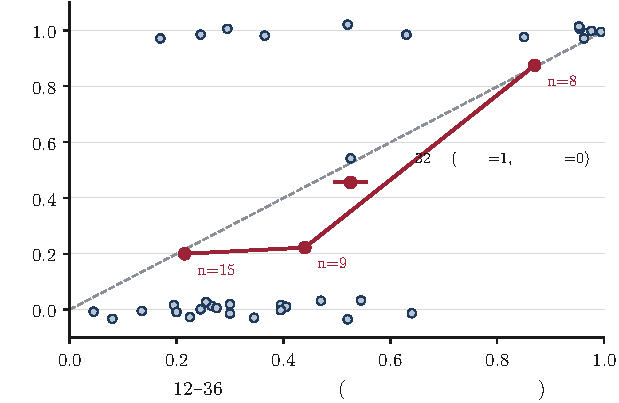
\includegraphics[width=0.64\textwidth]{fig/pm_calib.pdf}
\caption{예측시장 가격과 실제 실행 여부. 점선은 완전한 보정을 뜻한다.}\label{f:pmcal}
\end{figure}

시장은 이 계약들에 평균 0.44의 확률을 매겼고 실제로는 38\%가 실행됐다(표~\ref{t:pm}, 그림~\ref{f:pmcal}). 발효가 임박한 계약을 빼고 일주일 이상 존속한 계약만 보면 평균 가격 0.39, 실행 비율 0.31이다. 가격이 낮은 구간과 높은 구간은 잘 맞고, 가운데 구간에서 실행을 과대평가했다. 시장은 위협을 믿지 않은 것이 아니다. 실행 확률을 열에 셋에서 넷 정도로 매겼고, 그 값은 사후의 실행 비율과 크게 다르지 않았다. 5절의 작은 가격 반응은 이 숫자와 정합적이다.

같은 자료로 사건 시점의 믿음 변화도 볼 수 있다(그림~\ref{f:pmjump}). 위협과 직접 대응하는 계약이 게시 전에 이미 거래되던 경우, 위협은 계약 가격을 19--75\pp 올렸다. 2월 27일 대중 추가 관세 예고는 관련 계약을 0.22에서 0.76으로, 9월 25일 의약품 관세 예고는 0.13에서 0.88로 올렸다. 철회 직전의 가격은 낮았다. EU 50\% 계약은 연기 발표 직전 0.20, 한국 25\% 계약은 합의 직전 0.25, 그린란드 관세 계약은 철회 직전 0.40이었다. 시장은 명시적 번복이 나오기 전에 이미 실행 가능성을 낮게 보고 있었고, 번복은 남은 20--40\%를 지웠다.

\begin{figure}[H]
\centering
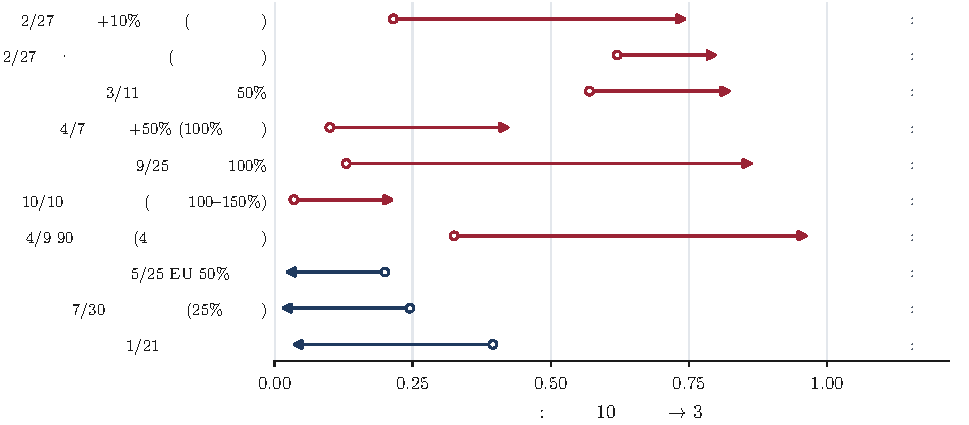
\includegraphics[width=0.82\textwidth]{fig/pm_jumps.pdf}
\caption{사건 시점의 예측시장 가격 변화. 화살표는 게시 10분 전 가격에서 3시간 뒤 가격으로 향한다. 붉은색은 강화 위협, 남색은 완화·철회다.}\label{f:pmjump}
\end{figure}

의약품 사례는 6.1절의 측정 한계를 다시 보여 준다. 실행 확률이 75\pp 뛰었는데 S\&P 500의 표준화 반응은 0.21이었다. 믿음은 크게 움직였지만 시장 전체에 대한 손실 $L$이 작았던 것이다. 가격 반응이 작다는 것만으로 위협을 믿지 않았다고 결론 내릴 수 없다.

\subsection{반응이 실리는 곳과 남는 시간}

위협과 철회는 서로 다른 시장에 실렸다(표~\ref{t:chan}). 강화 위협 때는 대상국 통화의 반응(평균 1.17)이 S\&P 500(0.43)보다 컸고, 철회 때는 S\&P 500만 움직였다($-1.63$ 대 $-0.10$). 위협은 특정 국가에 대한 뉴스로, 철회는 미국 정책 불확실성의 해소로 읽혔다는 해석이 가능하다.

\begin{table}[H]
\caption{반응의 경로와 지속성}\label{t:chan}
\tablefont
\begin{tabularx}{\textwidth}{@{}Yrrrr@{}}
\toprule
\multicolumn{5}{@{}l}{(가) 시장별 평균 표준화 반응}\\
 & S\&P 500 & 대상국 통화 & & \\
\midrule
강화 위협 & $0.43$ & $1.17$ & & \\
완화·철회 & $-1.63$ & $-0.10$ & & \\
예정 발효 & $0.43$ & $-0.08$ & & \\
\midrule
\multicolumn{5}{@{}l}{(나) 강화 위협 이후 S\&P 500 선물의 누적 변화 (중앙값, \%)}\\
 & 30분 & 1일 & 3일 & 10일\\
\midrule
19건 (4/9 제외) & $-0.11$ & $0.00$ & $+0.34$ & $+0.50$\\
\bottomrule
\end{tabularx}
\tnote{주: (가)의 통화 반응은 대상국 통화가 있는 사건만으로 계산했다(강화 10건, 완화 8건, 발효 9건). (나)는 추세를 조정하지 않은 기술통계다.}
\end{table}

전형적인 위협의 발표효과는 오래 남지 않았다. 위협 이후 S\&P 500 선물의 중앙값 변화는 30분에 $-0.11$\%, 하루 뒤 0.00\%, 사흘 뒤 $+0.34$\%다. 예외는 주요 교역국을 겨냥한 소수의 사건이다. 10월 10일 대중 위협 뒤 하루 동안 선물은 3.0\% 떨어졌다. 위협과 철회가 짝을 이루는 세 사례에서 30분 반응은 EU 50\%가 $-1.22$\%와 $+0.28$\%, 그린란드 관세가 $-0.67$\%와 $+1.13$\%, 대중 100\%가 $-1.51$\%와 $+0.78$\%였다.

\subsection{두 가지 경로}

큰 반응과 미실행이 함께 나타나는 데에는 두 가지 설명이 가능하다. 첫째는 협상 카드 경로다. 주요 교역국을 향한 큰 위협은 처음부터 협상을 위한 것이고, 시장은 실행 확률이 아니라 판돈의 크기에 반응한다. 둘째는 시장이 부른 후퇴 경로다. 가격이 크게 흔들리면 발표자가 물러난다. 2025년 4월 9일의 유예와 2026년 1월의 그린란드 관세 철회는 시장 급락 직후에 나왔다. 두 경로는 모두 반응이 클수록 실행되지 않는다고 예측하므로 이 자료로는 가를 수 없다. 둘째 경로가 맞다면 위협의 발표효과는 스스로를 무효화하는 성격을 갖는다. 이를 가르려면 위협 이후의 가격 경로와 번복 시점의 관계를 더 많은 사건에서 봐야 한다.

실행률 자체도 맥락 속에서 봐야 한다(표~\ref{t:bench}). 위협이 조치로 이어지는 비율은 법적 절차를 갖춘 통상 위협에서도 낮았다. 본 연구의 22--34\%는 제재 전반의 60\%보다 낮지만 301조의 13\%보다 높다. 낮은 실행률은 이 발표자만의 특징이라기보다 강압적 통상정책의 일반적 성격에 가깝고, 달라진 것은 위협의 빈도와 공개성이다.

\begin{table}[H]
\caption{위협이 조치로 이어진 비율}\label{t:bench}
\tablefont
\begin{tabularx}{\textwidth}{@{}YL{0.3\textwidth}r@{}}
\toprule
자료 & 대상 & 비율\\
\midrule
TIES (Morgan et al., 2014) & 경제제재 1,412건, 1945--2005 & 60\%\\
Bayard and Elliott (1994) & 미국 301조 91건, 1975--1994 & 13\%\\
Bloomberg Economics (2026) & 2025년 이후 관세 위협 & 약 25\%\\
본 연구 & 강화 위협 32건 & 22\% (부분 포함 34\%)\\
\bottomrule
\end{tabularx}
\tnote{주: TIES의 60\%는 위협 없이 바로 부과된 사례를 포함한 전체 사건 대비 부과 비율이다. 301조의 13\%는 일방적 보복이 단행된 12건의 비율이다. 정의가 서로 달라 직접 비교에는 주의가 필요하다.}
\end{table}

정리하면 이렇다. PMCCF는 발표자의 신뢰가 높아 실행 없이도 말이 가격을 움직인 사례다. 관세 위협은 실행 실적이 낮은데도 말이 가격을 움직인 사례다. 두 경우에 공통된 것은 실행 실적이 아니라 실행할 수 있는 능력과 실행됐을 때의 손실 크기다. 시장은 낮은 실행 확률을 대체로 맞게 매겼고, 그 확률에 손실 크기를 곱한 만큼 반응했다.

\section{확장: 수출통제 예고와 자본의 방향}

처음의 질문은 통제 예고가 대상국의 연구 자본을 옮기는가였다. 실제 연구개발 지출은 연간 자료라 사건 시점과 맞출 수 없고, 3절의 식별 문제가 그대로 남는다. 여기서는 그 앞 단계만 본다. 통제가 예고되거나 번복될 때, 자본이 국산 대체 쪽으로 옮겨 갈 것이라는 기대가 가격에 나타나는가.

2022년 10월부터 2026년 9월까지 미국의 대중 반도체·인공지능 수출통제 사건 17건을 모았다. 통제 강화 10건, 완화·번복 6건, 두 방향이 같은 날 나온 1건이다. 강화 10건 중 5건은 나중에 번복되거나 실행되지 않았다. H20 칩 허가제(2025년 4월)는 석 달 뒤 풀렸고, 설계 소프트웨어 허가제(5월)는 6주 뒤 철회됐으며, 계열사 규칙(9월)은 6주 뒤 유예됐다. 결과 변수는 중국의 국산 대체 기업 12개사(파운드리, 장비, 설계, 설계 소프트웨어)의 지수 대비 초과수익에서 미국 공급사 10개사의 S\&P 500 대비 초과수익을 뺀 값이다. 중국 본토와 홍콩 시장은 미국 장중에 닫혀 있으므로 사건 다음 거래일의 일별 수익률을 쓴다.

\begin{table}[H]
\caption{수출통제 사건 다음 거래일의 초과수익 (\%)}\label{t:xc}
\tablefont
\begin{tabularx}{\textwidth}{@{}Yrrrrr@{}}
\toprule
 & 건수 & 중국 국산 대체 & 미국 공급사 & 차이 & $t$\\
\midrule
통제 강화, 2022--2024년 & 3 & $-1.90$ & $-0.66$ & $-1.24$ & $-0.73$\\
통제 강화, 2025년 이후 & 7 & $2.17$ & $-0.54$ & $2.71$ & $2.14$\\
완화·번복, 2025년 이후 & 6 & $-1.54$ & $0.71$ & $-2.25$ & $-1.94$\\
\bottomrule
\end{tabularx}
\tnote{주: 동일가중 평균이다. 2025년 이후 강화 7건과 완화 6건의 차이에 대한 순위합 검정 $p=0.022$. 출처가 하나뿐인 2026년 5월 사건을 빼면 강화 6건의 차이는 3.74($t=4.25$)다. 사건 목록은 부록에 있다.}
\end{table}

\begin{figure}[H]
\centering
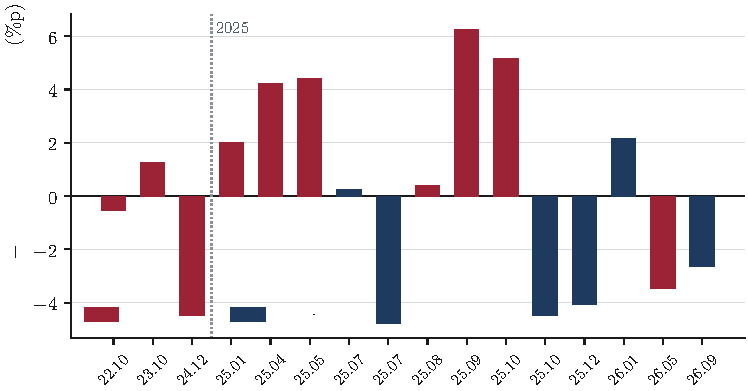
\includegraphics[width=0.8\textwidth]{fig/xc_spread.pdf}
\caption{수출통제 사건별 상대수익. 중국 국산 대체 기업의 초과수익에서 미국 공급사의 초과수익을 뺀 값이다.}\label{f:xc}
\end{figure}

2025년 이후에는 방향이 가설과 맞는다(표~\ref{t:xc}, 그림~\ref{f:xc}). 통제가 예고되면 중국 국산 대체 기업이 미국 공급사보다 평균 2.7\pp 더 올랐고, 번복되면 2.3\pp 더 내렸다. 두 집단의 차이는 순위합 검정으로 $p=0.022$다. 2022--2024년의 세 사건에서는 부호가 반대였다. 통제가 나오면 중국 기업도 함께 떨어졌다. 통제가 중국 기업에 대한 타격으로 읽히던 시기에서 국산화의 기회로 읽히는 시기로 넘어간 것처럼 보이지만, 이 구분은 결과를 보고 한 것이고 앞 시기는 3건뿐이다.

이 결과의 범위는 좁다. 표본은 16건이고, 가장 큰 두 건(2025년 9월 29일과 10월 10일)은 같은 시기의 중국 반도체 주가 상승 및 관세 충격과 겹친다. 주가는 기대된 자본 이동이지 실제 이동이 아니다. 말할 수 있는 것은 시장이 통제 예고를 자본이 국산 대체로 향할 신호로 가격에 반영한 것으로 보이며, 번복은 그 반영을 되돌렸다는 데까지다. 예고만으로 실제 연구개발 지출이 옮겨 갔는지는 본 연구가 답하지 못한 질문으로 남는다.

\section{결론}

실행되지 않는 위협도 시장을 움직인다. 2025년 이후 미국의 관세 위협 20건 중 16건에서 가격은 위험회피 방향으로 움직였고, 철회에는 반대 방향으로 반응했으며, 그 크기는 표본 기간인 약 1년 동안 줄지 않았다. 반응은 작았다. 예측시장이 매긴 실행 확률은 평균 0.4 안팎이었고 사후의 실행 비율과 대체로 맞았다. 발효일에는 새 정보가 도착하지 않았다. 정보는 말이 나오는 순간과 거둬지는 순간에 도착했다.

시장은 위협을 한 덩어리로 믿거나 의심한 것이 아니라 가려 들었다. 협상의 대상이 될 만한 큰 위협에는 크게 반응했고, 조용히 사라질 위협은 시장 전체 지표에서 거의 반응이 없었다. 미실행에는 통한 위협과 무시된 위협이 섞여 있으므로 실행률은 신뢰도의 척도가 아니다. 발표효과가 성립하는 데 필요한 것은 실행 실적이 아니라 실행 능력과 판의 크기라는 것이 본 연구의 해석이다.

한계는 분명하다. 시각을 확인한 사건이 강화 20건, 완화 9건, 발효 11건이어서 집단 간 비교의 검정력이 낮고, 차이가 없다는 결과는 차이를 찾지 못했다는 뜻이다. 6절과 7절의 분류와 분석은 사후적이다. 위협의 시점은 시장 상황에 내생적일 수 있고, 큰 반응이 후퇴를 부른 것인지 협상용 위협에 크게 반응한 것인지는 가르지 못했다. 서한과 발언으로 나온 위협은 빠져 있다. 품목 관세의 반응은 품목별 가격으로 다시 재야 한다. 2018--2019년과의 비교, 그리고 예고가 실제 연구개발 지출을 옮겼는지는 후속 과제다.

\section*{참고문헌}
\begingroup\small\setlength{\parindent}{0pt}\setlength{\parskip}{3pt}\RaggedRight
\newcommand{\bibitemx}{\hangindent=1.5em\hangafter=1 }
\bibitemx Altavilla, C., D. Giannone and M. Lenza (2016), ``The Financial and Macroeconomic Effects of the OMT Announcements,'' \textit{International Journal of Central Banking}, 12(3), 29--57.\par
\bibitemx Amiti, M., M. Gomez, S. H. Kong and D. E. Weinstein (2021), ``Trade Protection, Stock-Market Returns, and Welfare,'' NBER Working Paper 28758.\par
\bibitemx Bayard, T. O. and K. A. Elliott (1994), \textit{Reciprocity and Retaliation in U.S. Trade Policy}, Institute for International Economics.\par
\bibitemx Bloomberg Economics (2026), 관세 위협 실행 집계, \textit{South China Morning Post} 보도.\par
\bibitemx Gürkaynak, R. S., B. Sack and E. T. Swanson (2005), ``Do Actions Speak Louder Than Words? The Response of Asset Prices to Monetary Policy Actions and Statements,'' \textit{International Journal of Central Banking}, 1(1), 55--93.\par
\bibitemx Haddad, V., A. Moreira and T. Muir (2021), ``When Selling Becomes Viral: Disruptions in Debt Markets in the COVID-19 Crisis and the Fed's Response,'' \textit{Review of Financial Studies}, 34(11), 5309--5351.\par
\bibitemx Han, P., W. Jiang and D. Mei (2024), ``Mapping U.S.--China Technology Decoupling: Policies, Innovation, and Firm Performance,'' \textit{Management Science}, 70(12).\par
\bibitemx Hayakawa, K. and C.-H. Yang (2026), ``Technology Sanctions and Firm R\&D: Evidence From the U.S.--China Trade Dispute,'' \textit{Economics \& Politics}, 38(2), 406--419.\par
\bibitemx Hu, H., S. Yang, L. Zeng and X. Zhang (2024), ``U.S.--China Trade Conflicts and R\&D Investment: Evidence from the BIS Entity Lists,'' \textit{Humanities and Social Sciences Communications}, 11, 829.\par
\bibitemx Kalemli-Özcan, Ṣ., C. Soylu and M. A. Yildirim (2026), ``Tariff Uncertainty and the U.S. Dollar,'' NBER Working Paper 34728.\par
\bibitemx Krishnamurthy, A. and A. Vissing-Jorgensen (2011), ``The Effects of Quantitative Easing on Interest Rates: Channels and Implications for Policy,'' \textit{Brookings Papers on Economic Activity}, Fall, 215--287.\par
\bibitemx Liu, X., Y. Liu, A. Makarin and J. Wen (2025), ``Export Controls and Innovation in Sanctioned Countries,'' CEPR Discussion Paper 20690.\par
\bibitemx Ma, X., Y. Ma, H. Tao and Y. Zhang (2025), ``Market Contraction and Innovation Divergence: The Impact of the US--China Trade War on Chinese Innovation,'' PHBS Working Paper 20251106.\par
\bibitemx Merendino, A. and T. Monacelli (2026), ``Tariffs, Uncertainty, and the Exchange Rate,'' \textit{Economic Policy: Papers on European and Global Issues}, 학술대회 발표본.\par
\bibitemx Morgan, T. C., N. Bapat and Y. Kobayashi (2014), ``Threat and Imposition of Economic Sanctions 1945--2005: Updating the TIES Dataset,'' \textit{Conflict Management and Peace Science}, 31(5), 541--558.\par
\bibitemx Yale Program on Financial Stability, ``Primary and Secondary Market Corporate Credit Facilities,'' 사례 연구.\par
\endgroup

\appendix
\section*{부록 A. 게시 시각을 확인한 강화 위협}
\begingroup\footnotesize\linespread{1.08}\selectfont
\begin{tabularx}{\textwidth}{@{}llL{0.25\textwidth}L{0.15\textwidth}Yr@{}}
\toprule
날짜 & 시각(ET) & 대상 & 세율 & 결말 & $z$\\
\midrule
25-01-26 & 13:28 & Colombia & 25$\rightarrow$50\% & 미실행 (상대 양보) & $2.33$\\
25-02-27 & 08:46 & Mexico, Canada, China & 25, 25, +10\% & 실행 & $0.96$\\
25-03-11 & 10:15 & Canada steel/aluminum & 50\% & 미실행 (상대 양보) & $1.76$\\
25-03-13 & 07:58 & EU wine/spirits & 200\% & 미실행 (상대 양보) & $0.17$\\
25-03-24 & 10:37 & Buyers of Venezuelan oil & 25\% & 미실행 (일방 보류·소멸) & $-0.36$\\
25-04-07 & 11:14 & China & +50\% & 실행 & $1.38$\\
25-04-09 & 13:18 & China & 125\% & 실행 & $-4.74$\\
25-05-04 & 19:18 & Foreign films & 100\% & 미실행 (일방 보류·소멸) & $0.24$\\
25-05-23 & 07:43 & EU & 50\% & 미실행 (협상 타결) & $2.37$\\
25-05-30 & 19:16 & Steel/aluminum & 50\% & 실행 & $0.36$\\
25-07-09 & 20:29 & Copper & 50\% & 부분 실행 & $0.08$\\
25-07-30 & 08:09 & India & 25\%+벌칙 & 실행 & $0.04$\\
25-08-25 & 20:31 & Digital-tax countries &  & 미실행 (일방 보류·소멸) & $1.22$\\
25-09-25 & 18:51 & Heavy trucks & 25\% & 미실행 (일방 보류·소멸) & $0.36$\\
25-09-25 & 19:24 & Branded pharmaceuticals & 100\% & 미실행 (일방 보류·소멸) & $0.21$\\
25-10-10 & 10:57 & China & 대폭 인상 & 미실행 (협상 타결) & $5.45$\\
25-10-10 & 16:50 & China & +100\% & 미실행 (협상 타결) & $-1.25$\\
25-10-25 & 16:30 & Canada & +10\% & 미실행 (일방 보류·소멸) & $-0.13$\\
25-12-08 & 17:55 & Mexico & 5\% & 미실행 (상대 양보) & $0.36$\\
26-01-17 & 11:19 & Denmark+7 European & 10$\rightarrow$25\% & 미실행 (협상 타결) & $0.94$\\
26-02-21 & 07:59 & Global & 10$\rightarrow$15\% & 미실행 (일방 보류·소멸) & \\
\bottomrule
\end{tabularx}
\endgroup
\tnote{주: 결말의 괄호는 6.1절의 사후 분류다. 마지막 사건은 게시 시각의 시간대를 확정하지 못해 반응을 재지 않았다.}

\section*{부록 B. 수출통제 사건과 다음 거래일 초과수익 (\%)}
\begingroup\footnotesize\linespread{1.08}\selectfont
\begin{tabularx}{\textwidth}{@{}llYrr@{}}
\toprule
날짜 & 방향 & 조치 & 중국 대체 & 미국 공급사\\
\midrule
22-10-07 & 강화 & 첨단 컴퓨팅·반도체 장비 규칙(10/7 규칙) & $-3.96$ & $-3.43$\\
23-10-17 & 강화 & 10/7 규칙 강화(성능 밀도 기준) & $0.63$ & $-0.64$\\
24-12-02 & 강화 & 장비·HBM 통제+140개사 Entity List & $-2.37$ & $2.11$\\
25-01-13 & 강화 & AI 확산 규칙 발표(준수 시한 5/15) & $1.09$ & $-0.93$\\
25-04-15 & 강화 & Nvidia H20 허가 요건 공시 & $2.27$ & $-1.95$\\
25-05-13 & 혼합 & AI 확산 규칙 철회+화웨이 Ascend 지침 & $-2.70$ & $2.42$\\
25-05-28 & 강화 & EDA 소프트웨어 대중 판매 허가제(서한) & $2.31$ & $-2.10$\\
25-07-02 & 완화 & EDA 허가 요건 해제 & $0.93$ & $0.68$\\
25-07-14 & 완화 & H20 판매 재개 허용 & $-2.58$ & $2.19$\\
25-08-29 & 강화 & 삼성·SK하이닉스·인텔 중국 공장 VEU 철회 & $-1.36$ & $-1.75$\\
25-09-29 & 강화 & 계열사(50\%) 규칙 & $6.28$ & $0.02$\\
25-10-10 & 강화 & 트럼프: 핵심 소프트웨어 수출통제 11/1 예고 & $7.04$ & $1.88$\\
25-10-30 & 완화 & 부산 합의: 계열사 규칙 1년 유예 & $-5.14$ & $-0.67$\\
25-12-08 & 완화 & 트럼프: H200 대중 판매 허용 & $-3.59$ & $0.48$\\
26-01-13 & 완화 & H200 사안별 심사 규칙 & $2.54$ & $0.36$\\
26-05-31 & 강화 & 해외 소재 중국계 기업 첨단 칩 허가 지침 & $-2.41$ & $1.05$\\
26-09-23 & 완화 & 휴전·계열사 규칙 유예 2027-01-10까지 연장 발표 & $-1.40$ & $1.23$\\
\bottomrule
\end{tabularx}
\endgroup
\tnote{주: 날짜는 시장이 처음 반응할 수 있었던 보도·공시일이다. 중국 국산 대체 12개사는 SMIC(홍콩·상하이), 화훙, 북방화창, 중웨이, 캠브리콘, 하이곤, 웨이얼, 란치, 화다주톈, 화하이칭커, 퉈징이고 본토 종목은 CSI 300, 홍콩 종목은 항셍지수 대비 초과수익이다. 미국 공급사 10개사는 Nvidia, AMD, Applied Materials, Lam Research, KLA, Synopsys, Cadence, Micron, Qualcomm, Intel이다.}

\section*{부록 C. 예측시장 계약 32건}
\begingroup\scriptsize\linespread{1.05}\selectfont
\begin{tabularx}{\textwidth}{@{}lYrl@{}}
\toprule
상장일 & 계약 질문 (Polymarket) & 가격 & 결과\\
\midrule
24-11-26 & Will Trump impose 25\% tariff on Mexico or Canada before February? & $0.34$ & 아니오\\
25-02-04 & Trump tariffs on Canada in effect by May 1? & $0.36$ & 예\\
25-02-04 & Trump tariffs on Mexico in effect by May 1? & $0.52$ & 예\\
25-02-10 & 25\% aluminum tariff in effect before May? & $0.95$ & 예\\
25-02-10 & 25\% steel tariff in effect before May? & $0.96$ & 예\\
25-03-03 & Will Trump 10\% China tariff increase go into effect by Friday? & $0.99$ & 예\\
25-04-03 & Will Trump 10\% blanket tariff go into effect by Saturday? & $0.98$ & 예\\
25-04-04 & 54\% tariff goes into effect on China by Wednesday? & $0.85$ & 예\\
25-04-09 & Trump imposes 200\% tariff on China before June? & $0.20$ & 아니오\\
25-04-14 & Trump imposes tariff on pharmaceuticals before May? & $0.23$ & 아니오\\
25-05-06 & Will Trump impose film tariff by Friday? & $0.04$ & 아니오\\
25-05-23 & 50\% tariff goes into effect on EU by June 1? & $0.24$ & 아니오\\
25-05-26 & 50\% tariff goes into effect on EU by July 9? & $0.14$ & 아니오\\
25-07-11 & 35\% Canada tariff in effect by August 1? & $0.29$ & 예\\
25-07-11 & 50\% Brazil tariff in effect by August 1? & $0.40$ & 아니오\\
25-07-11 & 25\% South Korea tariff in effect by August 1? & $0.47$ & 아니오\\
25-07-11 & 50\% copper tariff in effect by August 1? & $0.63$ & 예\\
25-07-11 & 25\% Japan tariff in effect by August 1? & $0.41$ & 아니오\\
25-07-14 & 30\% EU tariff in effect by August 1? & $0.27$ & 아니오\\
25-08-06 & 50\% India tariff in effect by August 27? & $0.24$ & 예\\
25-08-06 & Trump imposes tariff on pharmaceuticals by August 31? & $0.52$ & 아니오\\
25-08-07 & Trump imposes tariff on semiconductors by August 31? & $0.55$ & 아니오\\
25-08-27 & Trump imposes tariff on pharmaceuticals by September 30? & $0.30$ & 아니오\\
25-08-27 & Trump imposes tariff on semiconductors by September 30? & $0.64$ & 아니오\\
25-10-23 & Trump imposes tariff on semiconductors by December 31? & $0.26$ & 아니오\\
25-10-11 & 100\% tariff on China in effect by November 1? & $0.28$ & 아니오\\
26-01-18 & Will any of Trump's Greenland Tariffs go into effect by Feb 1? & $0.40$ & 아니오\\
26-01-24 & Tariff increase on Canada in effect by June 30? & $0.30$ & 아니오\\
26-01-24 & 100\% tariff on Canada in effect by June 30? & $0.08$ & 아니오\\
26-02-20 & New 10\% US blanket tariff goes into effect by February 28? & $0.95$ & 예\\
26-09-10 & Will Trump raise tariffs on Canada by September 15? & $0.20$ & 아니오\\
26-10-15 & Will Trump raise tariffs on Canada by October 31? & $0.17$ & 예\\
\bottomrule
\end{tabularx}
\endgroup

\section*{부록 D. 자료와 재현}
가격은 Dukascopy 1분봉(S\&P 500 지수 CFD, 주요 통화쌍)과 Yahoo Finance(일별·시간별 주가, 선물)이며, 예측시장 자료는 Polymarket의 공개 가격 이력이다. 게시 시각은 American Presidency Project의 Truth Social 기록, 위협의 결말은 관세 추적 자료와 통신사 연표에서 확인했다. 사건 목록, 분석계획(v1, v1.1), 수집·분석 코드, 사건별 반응은 저장소에 있다. 분석계획과 사건 목록은 가격 열람 전에 고정했고, 그 뒤의 변경(수출통제 사건 1건의 날짜 정정 등)은 변경 이력에 기록했다.
\end{document}
